\subsection{Resize}
Resizing an already rotated object would result in an odd and unintuitive behaviour.
The problem was that the dragged vector just added its dimensions to the rectangles width and height.
However, if the rectangle is rotated, the dragged vector would still add its dimensions to the rectangle as if the rectangle was not rotated.
This issue would for example have a opposite resizing if the rectangle was rotated $90\deg$, as can be seen in \figref{fig:resizeRotate}.\fxwarning{look at the figures again, make sure they are detailed enough}
\begin{figure}
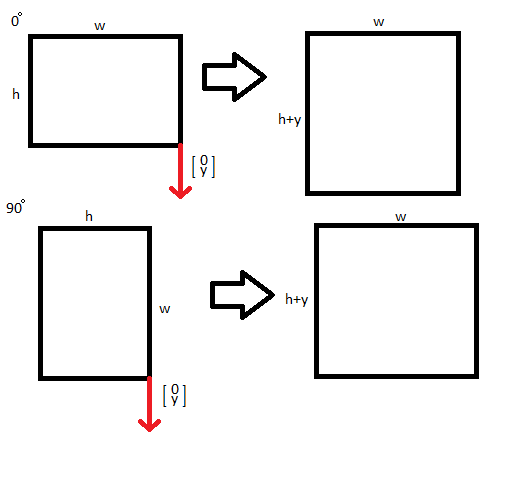
\includegraphics[scale=0.5]{media/How-Rotate+Resize-Worked}
\caption{Example showing previous resize rotate combination}
\label{fig:resizeRotate}
\end{figure}
%Kan godt være den her linie skal skrives lidt om
To change this behaviour we tried some different ideas, which resulted in failure but will still be documented to show our effort towards this issue. 

%1: rotate then apply
The initial approach was to rotate the vector with the same angle as the rectangle is rotated and then apply the dimensions as previously.
However, this approach was mathematically flawed as the vector could end up with negative dimensions after rotation and decrease the size of the rectangle where the motion of the user intuitively should increase the size of the rectangle.

%2: rotate around a "pivot"
In an attempt to reuse the idea in the previous approach, we realised that the rotation of the vector should be around a specific line in 3D.
An example to show this idea could be shown using $\vec{a} =
\begin{bmatrix}
2 \\ 3
\end{bmatrix}$, and let us say the rectangle is rotated by $90\deg$.
This means the vector has to be rotated $180^\circ$ around a line that is tilted $45^\circ$, as illustrated in \figref{fig:app2}, resulting in a new vector 
$\begin{bmatrix}
3 \\ 2
\end{bmatrix}$.
\begin{figure}
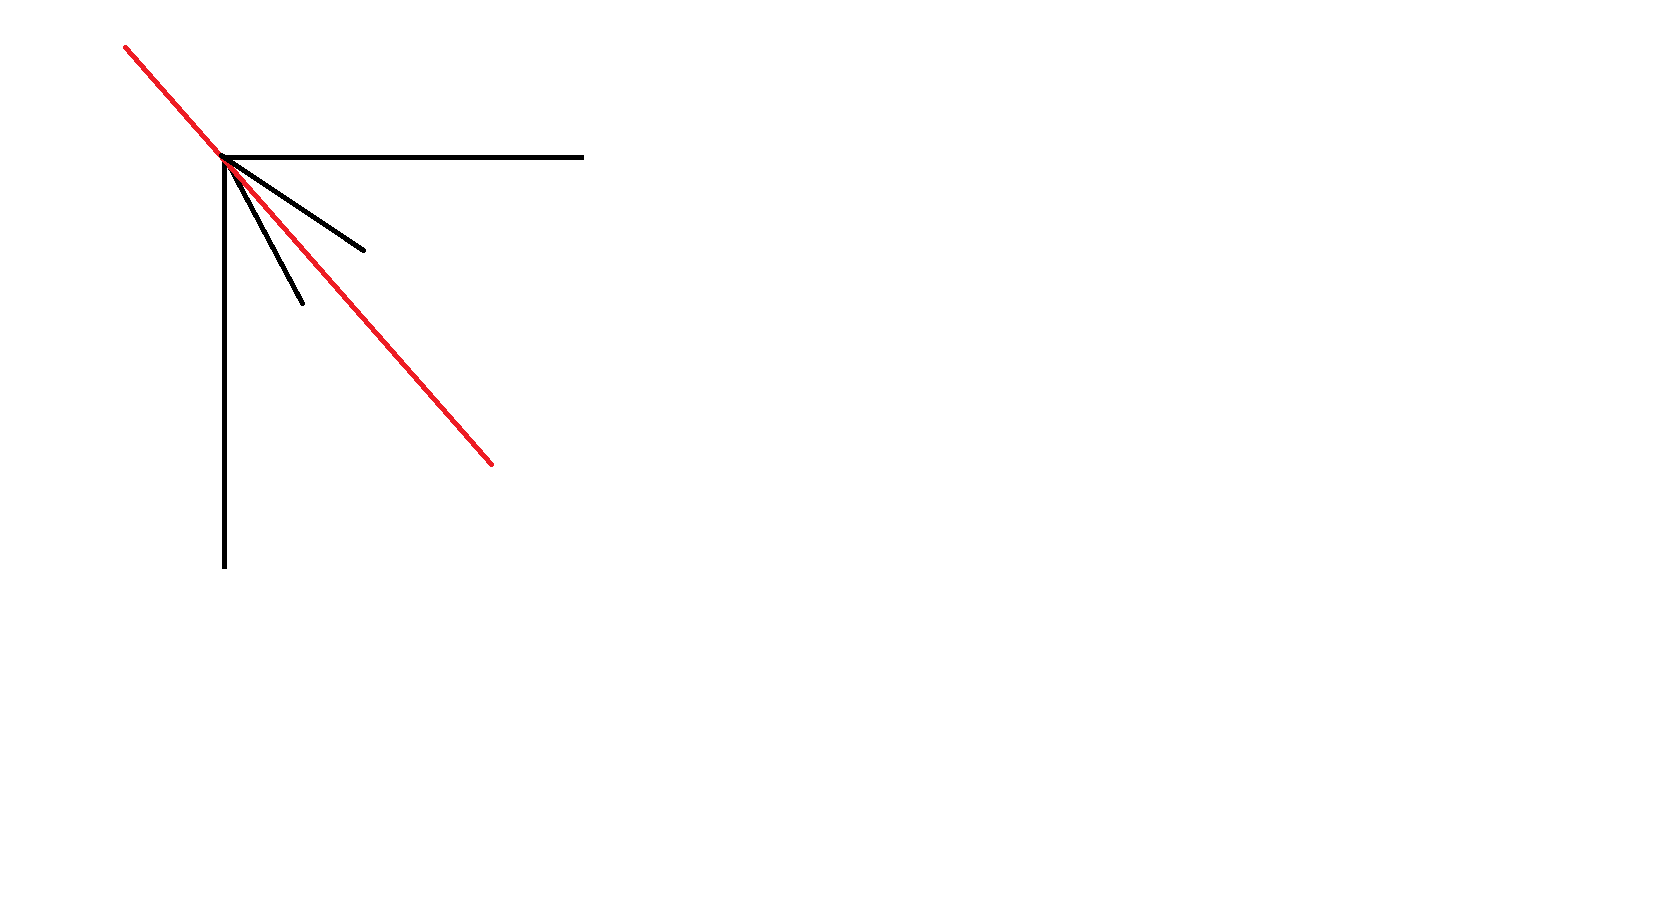
\includegraphics[scale=0.5]{media/approach2}
\caption{Example showing 2nd resize approach}
\label{fig:app2}
\end{figure}
The problem with this approach was that we could not mathematically express where the line should be  for the general case.
We believe that if this line could be determined, this approach would be sufficient to solve this issue.
However, we would also have to examine how much we should rotate around the to be determined line.

%3: scale as much as hitbox grows
Since we could not find that line, we decided to take another approach and instead of looking at the drag vector, we look at how the hitbox changes. 
The drag vector was now applied to the hitbox and we looked at how much the hitbox would change in size.
This size change would then be applied to the rectangle inside the hitbox, but had the same problems as in the original problem as when the rectangle is rotated above $90^\circ$ its heigth should be changed when the hitbox width was changed.

%4: resize hitbox, keep smaller rect. properties/dimension
Next approach expanded upon the idea of using the hitbox. 
We looked at where the edges of the rectangle connected with the hitbox and when the dimensions of the hitbox changed, we place these edges at the same ratios.
For example, assume that the an edge of the rectangle connected with the hitbox with a ratio of $20\% - 80\%$, it should keep that ratio after the hitbox was resized.
However, this approach would conceptually stretch the rectangle instead of resizing it, resulting in it no longer being a rectangle.
This result could not be represented on the android device as the object was considered a rectangle at all times, due to this, it was never implemented.
\begin{figure}
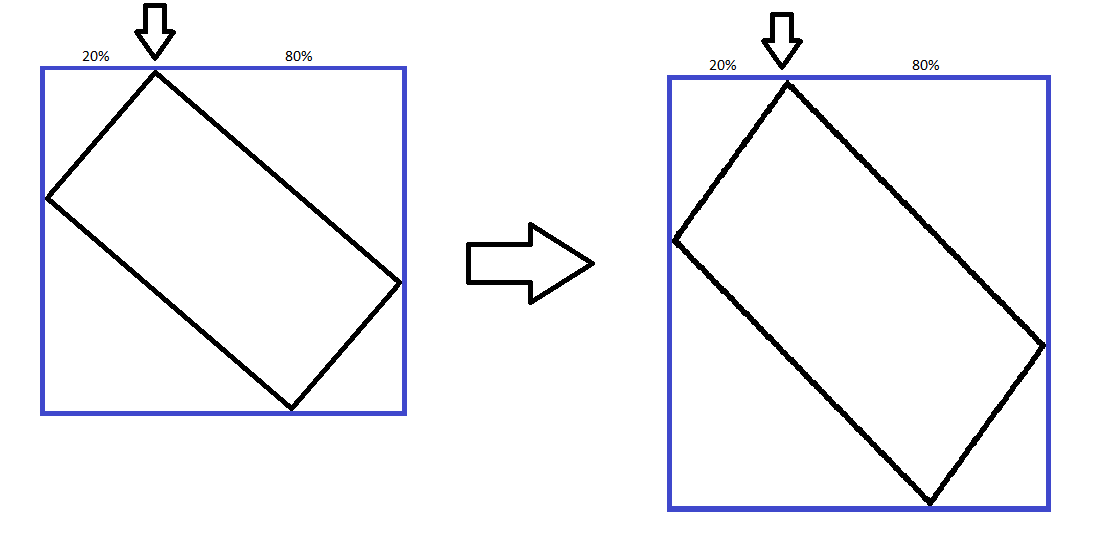
\includegraphics[scale=0.5]{media/approach4}
\caption{Example showing 4th resize approach}
\label{fig:app4}
\end{figure}

%5: width and height to vectors and resize acordingly.
Yet again we took the idea in another direction, and looked at the width and height of the rectangle as vectors.
The angle of these vectors would be divided by the angle of the drag vector, to find a factor of how much each side had to be affected.
For example, let us assume that the width vector has an angle of $60^\circ$, the height vector an angle of $150^\circ$, and the drag vector $30^\circ$.
The factor would then be found as follows:
\begin{equation}
\begin{aligned}
w' = v / w\\
h' = 1 - w'\\
\end{aligned}
\end{equation}
where, 
\begin{itemize}
\item[$w$] is the angle of the width vector.
\item[$v$] is the angle of the drag vector.
\item[$w'$] is the factor of much the width should be affected.
\item[$h'$] is the factor of how much the height should be affected.
\end{itemize}
The equation would be opposite when the angle of the width vector was above $90^\circ$.
With the above example the factors would be $w' = 0.5$ and $h' = 0.5$, which means half the length of the drag vector will be added to the width and height.
A problem occurs when the angle of the width vector would be a lot smaller or larger than the drag vector angle and for example add twice the length of the drag vector.

%Current solution
The current and possibly final approach is to reset the starting point of the rectangle and swap the width and height.
This happens when the rotation angle of the rectangle is between $45^\circ$ and $315^\circ$, which is corresponds to the possible angles to be between $45^\circ$ and $-45^\circ$.
We implemented this approach since we observed that the resizing was reasonably accurate as long as the rotation angle was below $45^\circ$.
As an example, let the rotation of the rectangle be $46^\circ$, this means the dimensions of the rectangles are swapped and the rotation angle is sat to $-44^\circ$, as can be seen in \figref{fig:app6}.
\begin{figure}
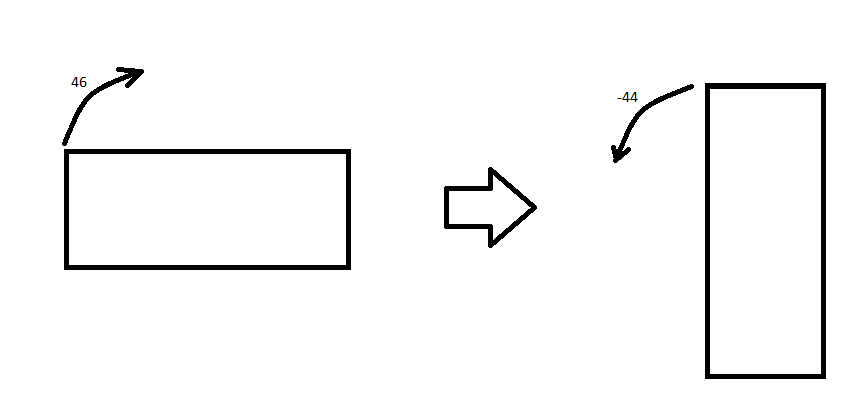
\includegraphics[scale=0.5]{media/approach6}
\caption{Example showing the current and possibly final resize approach}
\label{fig:app6}
\end{figure}
